%Tipo de documento
\documentclass[a4paper,12pt,twoside]{article} %book, report, letter, beamer

%Paquetes

%Configuracion inicial
\usepackage[utf8]{inputenc}
%\UseRawInputEncoding
\usepackage[spanish]{babel}
%Hipervinculos dinamicos
\usepackage[backref]{hyperref}
%Matematicas
\usepackage{amssymb}
\usepackage{amsmath}
\usepackage{amsbsy}
%Comentarios de varias lineas
\usepackage{comment}
%Insertar imagenes
\usepackage{graphicx}
\graphicspath{ {IMAGENES/} }
%Cuadros de codigo
\usepackage{listings}



% Cuerpo del documento -------------------------------------------------
%Entorno: comando especial que cuenta con parte de incio y de fin.

\begin{document}

%Portada
\begin{titlepage}
\centering

{
\includegraphics[width=0.6\textwidth]{foto_portada.png}\par}
\vspace{1cm}

{\bfseries\LARGE Escuela Técnica Superior de Ingeniería Informática y Telecomunicaciones \par}
\vspace{0.4cm}

{\scshape\Huge Exploración de Grafos \par}
\vspace{0.4cm}

{\itshape\Large Cuarta Práctica de Algorítmica \par}
\vspace{0.5cm}

{\itshape\Large Doble Grado en Ingeniería Informática y Matemáticas \par}
\vspace{0.4cm}

{\Large Autores: \par}
{\Large Elena Abreu Fernández \par}
{\Large Antonio Cantillo Molina \par}
{\Large Leandro Jorge Fernández Vega \par}
\vfill

{\Large Mayo 2023 \par}

\end{titlepage}

% Crea indice
\tableofcontents
\newpage


\section{Objetivos}


	\begin{itemize}
		\item Conocer en profundidad la implementación de un algoritmo de exploración de grafos: de tipo \textit{Backtracking} y \textit{Branch \& Bound}.
		\item Saber demostrar la optimalidad de una solución de un algoritmo \textit{Backtracking} y \textit{Branch \& Bound}.
		\item Abordar el diseño de funciones de cota.
		\item Aprender a utilizar recursos gráficos como GNUPLOT y aplicar conocimiento estadístico a los análisis.
	\end{itemize}
\newpage


\section{Introducción}

Se plantea la elaboración de un algoritmo de tipo \textit{Backtracking} y otro \textit{Branch \& Bound}. Estos algoritmos son de exploración de grafos y se usan para buscar varias secuencias de soluciones hasta encontrar la más óptima.\\

La idea básica es construir la tupla escogiendo
una componente cada vez, y usando funciones de criterio modificadas
$P_i(x_1,x_2,x_3,...,x_n)$., que a veces se llaman funciones de acotación o poda, para testear si la tupla que se está formando tiene posibilidad de éxito. La principal ventaja de este método es que si a partir de la tupla parcial $(x_1,...,x_i)$. se deduce que no se podrá construir una solución, entonces pueden ignorarse por completo el resto de combinaciones de tuplas.\\

Los algoritmos \textit{Backtracking} y \textit{BB} determinan las soluciones del problema buscando en el espacio de soluciones del caso considerado sistemáticamente. Esta búsqueda se facilita usando una organización en árbol para el espacio solución. Para un espacio solución dado, pueden caber muchas organizaciones en árbol. 

\subsection{Características}

\begin{itemize}
    \item La solución debe poder expresarse mediante una tupla $(x_1,x_2,x_3,...,x_n)$.
    \item Unas veces el problema a resolver trata de encontrar una tupla que maximiza (o minimiza) una función criterio u objetivo $P(x_1,x_2,x_3,...,x_n)$.
    \item Otras veces solo se trata de encontrar una tupla que satisfaga (no optimice) el criterio.
    \item Otras veces se trata de encontrar todas las tuplas que satisfagan el criterio.
\end{itemize} 

\subsection{Elementos}

\begin{itemize}

	\item Solución parcial: tupla o vector al que aún no se han asignado todos sus componentes.
	\item Función de poda: función que permite saber cuando una solución parcial no conduce a una completa.
	\item Restricciones explícitas: reglas que restrigen el rango de valores que pueden ser parte de la solución.
	\item Restricciones implícitas: reglas que indican cuando una solución parcial nos puede llevar a una solución correcta.
	\item Árbol de estados: organización en forma de árbol del espacio de solución.
        \item Estado del problema: nodos del árbol.
        \item Estado solución: nodos que representan una posible solución.
        \item Estado respuesta: una solución del problema.
        \item Nodo vivo: nodo que ya ha sido generado pero no tiene todos sus hijos generados
        \item Nodo muerto: nodo que o bien ha sido podado o bien todos sus hijos han sido generados.
        \item E-nodo: nodo vivo del que se están generando descendientes.
      
        

\end{itemize}

\newpage


\subsection{Datos Técnicos del Computador Utilizado}

\begin{itemize}

	\item Nombre del dispositivo: ASUS LAPTOP-7LR09K87

	\item Procesador: 11th Gen Intel(R) Core(TM) i7-11370H @ 3.30GHz   3.30 GHz

	\item RAM instalada: 16,0 GB (15,7 GB usable)

	\item Tipo de sistema: Sistema operativo de 64 bits.

	\item Arquitectura: x86\_64

	\item Cachés: L1d: 48 KiB (1 instance), L1i: 32 KiB (1 instance), L2: 1.3 MiB (1 instance), L3: 12 MiB (1 instance)

\end{itemize}
\vspace{1cm}

\subsection{Tipos de Análisis a Realizar}

\subsubsection{Análisis Teórico}

Para determinar a qué orden de eficiencia teórico pertenece un algoritmo, consideramos las siguientes definiciones:

\begin{itemize}

	\item Caso Peor:\\
	\begin{math}
	T(n) \in O(f(n)) \Leftrightarrow \exists K \in \mathbb{R^+} , \exists n_0 \in \mathbb{N} : T(n) \leq K \cdot{f(n)} \ \ \forall n > n_0
	\end{math}
	
	\item Caso Exacto:\\
	\begin{math}	
	T(n) \in \Theta(f(n)) \Leftrightarrow \exists K \in \mathbb{R^+} , \exists n_0 \in \mathbb{N} : T(n) = K \cdot{f(n)} \ \ \forall n > n_0
	\end{math}
	
	\item Caso Mejor:\\
	\begin{math}
	T(n) \in \Omega(f(n)) \Leftrightarrow \exists K \in \mathbb{R^+} , \exists n_0 \in \mathbb{N} : T(n) \geq K \cdot{f(n)} \ \ \forall n > n_0
	\end{math}
	
\end{itemize}

\vspace{1cm}




\newpage
\subsubsection{Análisis Empírico}

El análisis empírico supone la ejecución del algoritmo de ordenación para diferentes tamaños del vector. Para ello, usaremos los siguientes recursos:\\


\begin{itemize}
	\item La biblioteca $<$chrono$>$ y sus funciones para medir tiempos.
	
	\lstset{language=C++}
	\begin{lstlisting}

#include <chrono>
	
high_resolution_clock::time_point t_antes, t_despues;
duration<double> transcurrido;

t_antes = high_resolution_clock::now();

algoritmo(a0,a1,...);

t_despues = high_resolution_clock::now();
transcurrido = 
duration_cast<duration<double>>(t_despues - t_antes);
cout << "el tiempo empleado es " 
<< transcurrido.count() << " s." << endl;
	
	\end{lstlisting}
	
\vspace{1cm}

	\item El siguiente script para automatizar la obtención de resultados para diferentes tamaños:

	\lstset{language=Bash}
	\begin{lstlisting}
#!/bin/bash 

i="inicio"
while [ "$i" -le "tope" ]
do
        generador salida.dat $i
 	algoritmo salida.dat >> salida.dat
        i=$(( $i + "salto" ))
done
      

	\end{lstlisting}
	
\end{itemize}

\newpage
\subsubsection{Análisis Híbrido}

Consiste en obtener las constantes ocultas de la función del algoritmo. Para ello, utilizamos la herramienta GNUPLOT. Pondremos como ejemplo un algoritmo cuadrático.\\

Primero deberemos introducir la ecuación de la que queremos obtener los coeficientes:\\

\fbox{gnuplot$>$ f(x) = a0*x*x+a1*x+a2}\\

Después le indicaremos a GNUPLOT que realice un ajuste por mínimos cuadrados, donde \textit{salida.dat} es el fichero de datos.\\

\fbox{gnuplot$>$ fit f(x) 'salida.dat' via a0,a1,a2}\\

La parte que más interesa es el apartado \textit{\textbf{Final set of parameters}}, donde se encuentra el valor de los parámetros.\\

Para graficar utilizamos:\\

\fbox{gnuplot$>$ 'salida.dat', f(x) title 'Curva de Ajuste'}\\

Para determinar la bondad del ajuste, podemos utilizar la varianza, aunque el propio análisis teórico y los resultados gráficos nos permiten confirmar que la ecuación parabólica y n-logarítmica representan buenas aproximaciones para los algoritmos a tratar.

\newpage

\section{Problema: El viajante de comercio (PVC)}

Una empresa que comercializa componentes informáticos ha contratado un nuevo comercial. Al agente le ha asignado un conjunto de clientes, facilitándole la información relevante de cada uno, que incluye nombre, correo electrónico, teléfono y dirección postal. El director comercial le encarga al nuevo agente visitar a todos esos clientes, con el objetivo de hacer buenas ventas y que no vuelva hasta que haya visitado a todos los clientes. Por tanto, el recorrido considerado debe comenzar y finalizar en la empresa. Además, sólo podrá visitar cada cliente una sola vez. Además, para reducir gastos de desplazamiento, la distancia total recorrida debe ser lo más corta posible.


\paragraph{Aclaración}
Este problema es de tipo NP-completo, lo que quiere decir que no se ha encontrado un algoritmo que encuentre la solución óptima en tiempo polinomial para instancias grandes del problema.\\

Para ello, hemos escogido la siguiente implemnatción:


\lstset{language=C++}
\begin{lstlisting}
/*
 * struct que encapsula el concepto de cliente de un 
   vendedor cualquiera.
 * @field x Coordenada x del cliente.
 * @field y Coordenada y del cliente.
 * @field id Identificador del cliente.
 */
struct cliente{
    double x;
    double y;
    int id;

    bool operator < (cliente cliente) const{
        return id<cliente.id;
    }
};


\end{lstlisting}
\newpage

\subsection{Generador}

Permite generar los ficheros con los datos a utilizar.\\

\subsubsection{Implementación}
\lstset{language=C++}
\begin{lstlisting}
#include <iostream>
#include <string>
#include <fstream>
#include <random>

using namespace std;

int main(int argc, char *argv[]) {

    // Comprobacion de argumentos
    if (argc != 3) exit(-1);

    // Tomamos argumentos
    string fichero = argv[1];
    int n_clientes = stoi(argv[2]);

    ofstream salida;
    salida.open(fichero);

    // Rellenamos el fichero con los datos de los clientes
    salida << n_clientes << endl;

    // Generar clientes con sus identificadores 
    // y coordenadas x e y.
    const int MIN=0, MAX=10;
    std::random_device rd;
    std::default_random_engine eng(rd());
    std::uniform_real_distribution<double> distr(MIN,MAX);

    for (int i = 0; i < n_clientes; i++) {
        salida << i << " " << distr(eng) << " " 
               << distr(eng) << endl;
    }

    // Cerramos el fichero y lo devolvemos.
    salida.close();
    return 0;
}

\end{lstlisting}


\subsection{BackTracking}
Esta técnica resuelve problemas de optimización realizando un búsqueda exhaustiva. Se basa en la idea de construir progresivamente una solución candidata verificando en cada paso que se cumplan todas las restricciones correspondientes y retrocediendo cuando la solución parcial no pueda extenderse a una solución válida.
Para resolver nuestro problema con BackTracking, hemos creado una clase PVC\_BT, en la que representamos la solución como un vector del struct clientes:\\

\subsubsection{Implementación}

\lstset{language=C++}
\begin{lstlisting}
class PVC_BT{
private:

    /*
     * @brief Valor que nos permite determinar que distancia total 
     tiene nuestra ruta solucion.
     */
    double cota_global;

    /*
     * @brief Ruta de clientes solucion.
     */
    vector<cliente> rutafinal;


    /*
    * @brief Vector que nos permite ir aniadiendo clientes para 
    obtener posibles soluciones.
    */
     
    vector<cliente> ruta_actual;

    /*
     * @brief Vector de clientes.
     */

    vector<cliente> clientes;

    /*
    * @brief Metodo que calcula la distancia euclidea entre 
      dos clientes.
    */

    double distancia(cliente cliente1, cliente cliente2){

        return sqrt(pow(abs(cliente1.x-cliente2.x),2) + 
        pow(abs(cliente1.y-cliente2.y),2));
    }


    /*
     * @brief Metodo que devuelve la posicion del minimo 
     en una fila determinada de una matriz de double.
     * @param matriz_dist Matriz de la que obtener la posicion 
     del minimo de la fila.
     * @param pos Fila de la que obtener la posicion del minimo.
     */

    int DevuelveMinimoFila
            (const vector<vector<double>>& matriz_dist,
            int pos){
        double min=INFINITY;
        int pos_min = 0;
        for(int i=0;i<matriz_dist[pos].size();++i){
            if(matriz_dist[pos][i]<min && !clientes[i].visitado){
                min = matriz_dist[pos][i];
                pos_min = i;
            }
        }
        return pos_min;
    }


    /*
     * @brief Metodo que devuelve la posicion del minimo de 
       una matriz de double.
     * @param matriz_dist Matriz de la que obtener la posicion del minimo.
     */

    int DevuelveMinimoGrafo(const vector<vector<double>>& matriz_dist){
        double min = INFINITY;
        int pos_min = 0;
        for(int i=0; i<matriz_dist.size();++i){
            if(matriz_dist[i][DevuelveMinimoFila(matriz_dist,i)]<min){
                min = matriz_dist[i][DevuelveMinimoFila(matriz_dist,i)];
                pos_min = i;
            }
        }
        return pos_min;
    };

public:

    /* @brief Contructor con parametros.
     * @param clientes Vector de clientes del que calcular 
     *        el mejor recorrido.
     */

    PVC_BT (vector<cliente> clientes){
        cota_global=DistanciaTotal(clientes);
        this->clientes=clientes;
        rutafinal=clientes;
    }




    /*
     * @brief Metodo que crea una matriz de distacias a partir 
     *        de un vector de clientes.
     * @param clientes Vector de clientes del que calcular 
     *        calcular las distancias de todos los clientes 
     *        con todos.
     */

    vector<vector<double>> CrearMatriz(const vector<cliente>& 
                                                    clientes){
                                                    
        vector<vector<double>> matriz_dist= 
        vector<vector<double>>(clientes.size(),
                               vector<double>(clientes.size()));
                               
        for(int i=0;i<clientes.size();++i){
            for(int j=i+1;j<clientes.size();++j){
                matriz_dist[i][j]= distancia(clientes[i],
                                             clientes[j]);
            }
        }
        
        return matriz_dist;
    }


    /*
     * @brief Devuelve el vector ruta solucion.
     */

    vector<cliente> getRutaFinal(){
        return this->rutafinal;
    }

    /*
     * @brief Calcula la distancia de una ruta de clientes.
     * @param ruta Vector de clientes del aque calcular 
     *        la distancia.
     */

    double DistanciaTotal(const vector<cliente>& ruta){
        double sol = 0;
        for(int i=0; i<ruta.size()-1; ++i){
            sol+= distancia(ruta[i],ruta[i+1]);
        }
        return sol;
    }

    /*
     * @brief Algoritmo basado en Backtracking para el Problema del 
     *        Viajante de Comercio.
     * @param pos_actual E-nodo sobre el que se trabaja. Es decir, 
     *        posible cliente que incluir en la ruta solucion.
     * @param dist_actual Longitud de la ruta que se esta construyendo.
     * @param matriz_dist Matriz de distancias de los clientes.
     * @param Cota Funcion que determina la optimalidad de las 
     *        soluciones que se van calculando.
     * @param Matriz de double que se correspondera con la matriz 
     *        de distancias.
     * @param Variable double que se correspondera con la 
     *        distancia acumulada.
     */

    void BT (int pos_actual, double dist_actual, 
             const vector<vector<double>>& matriz_dist, 
        double (PVC_BT::*Cota)(const vector<vector<double>>&,double)){


        if(dist_actual>((this->*Cota)(matriz_dist,dist_actual))) return;

        if(ruta_actual.size()==clientes.size()){
            dist_actual+=matriz_dist[pos_actual][ruta_actual.front().id];
            if(dist_actual<cota_global){
                cota_global=dist_actual;
                rutafinal=ruta_actual;
            }
            return;
        }

        for(int sig=0; sig<rutafinal.size();++sig){
            if(!rutafinal[sig].visitado){

                rutafinal[sig].visitado = true;
                clientes[rutafinal[sig].id].visitado=true;
                ruta_actual.push_back(clientes[rutafinal[sig].id]);

                BT(sig, DistanciaTotal(ruta_actual),matriz_dist,Cota);

                (find(rutafinal.begin(), rutafinal.end(),
                ruta_actual.back()))->visitado=false;
                clientes[ruta_actual.back().id].visitado=false;
                ruta_actual.pop_back();
            }
        }

    }
};

\end{lstlisting}

\vspace{1cm}

\subsubsection{Funciones de Cota}
\vspace{0.3cm}

\textbf{Primera Cota}\\

 Para esta primera cota elegimos como cota local el resultado de multiplicar el peso del menor arco por el número de ciudades que quedan por visitar, y a eso sumarle la distancia recorrida hasta el momento. Lo hemos implementado de la siguiente manera:\\

\lstset{language=C++}
\begin{lstlisting}
 /*
     * @brief Primer estimador para determinar la validez de 
       las posibles soluciones a lo largo de su construccion.
     * Selecciona el arco de menor peso y multiplica dicho peso 
       por el numero de ciudades que quedan por visitar.
     * @param matriz_dist Matriz de distancias.
     * @param dist_acumulada Distancia del recorrido ya hecho en 
       la exploracion del grafo.
 */

double FuncionCota1(const vector<vector<double>>& matriz_dist,
                      double dist_acumulada){

    double menor_peso =
        matriz_dist[DevuelveMinimoGrafo(matriz_dist)]
    [DevuelveMinimoFila
    (matriz_dist,DevuelveMinimoGrafo(matriz_dist))];
   int quedan_por_visitar = clientes.size() - ruta_actual.size();
        return (menor_peso*quedan_por_visitar)+dist_acumulada;
    }
\end{lstlisting}

\newpage
\textbf{Segunda Cota}\\

 A continuación, hemos creado la siguiente función para asignar a la cota local el resultado de sumarle a la distancia recorrida hasta el momento el mínimo valor de "salir" de cada nodo aún no visitado. La implementación es la siguiente:
 
\lstset{language=C++}
 \begin{lstlisting}

/*
     * @brief Segundo estimador para determinar la validez de las 
       posibles soluciones a lo largo de su construccion.
     * Selecciona el arco de menor peso al salir de todos los nodos
       restantes por visitar, y suma esto a la distancia
     * acumulada del camino ya recorrido.
     * @param matriz_dist Matriz de distancias.
     * @param dist_acumulada Distancia del recorrido ya hecho en la 
     exploracion del grafo.
*/

    double FuncionCota2(const vector<vector<double>>& matriz_dist,
                       double dist_acumulada){

        for (int i=0; i<matriz_dist.size();++i){
            if (!clientes[i].visitado){
             dist_acumulada+=matriz_dist[i]
             [DevuelveMinimoFila(matriz_dist,i)];
            } 
        }
        return dist_acumulada;
    }

\end{lstlisting}

\newpage
\textbf{Tercera Cota}\\

Para la tercera y última función se ha seguido el siguiente criterio: para cada arista se considera la mitad de su peso como el costo de salir y entrar, y, para las ciudades que aún no han sido visitadas, se considera la mitad de la suma de sus dos menores arcos. Se ha implementado como sigue:

\lstset{language=C++}
\begin{lstlisting}
/*
    * @brief Tercer estimador para determinar la validez de las
      posibles soluciones a lo largo de su construccion.
    * Selecciona el arco de menor peso al salir y entrar en cada
      nodo, dividiendo por 2.
    * @param matriz_dist Matriz de distancias.
    * @param dist_acumulada Distancia del recorrido ya hecho en la
      exploracion del grafo.
*/

 double FuncionCota3(const vector<vector<double>>& matriz_dist,
                    double dist_acumulada){
        vector<vector<double>> m=matriz_dist;
        double aux=0;
        double dist=0;
        double min1;

        if(ruta_actual.size()==0) dist=dist_acumulada;
        else if (ruta_actual.size()==1) {
            aux=distancia(ruta_actual[0], ruta_actual[1]);
            dist=(matriz_dist[ruta_actual[0].id]
            [DevuelveMinimoFila(matriz_dist,ruta_actual[0].id)] + 
                       aux)/2;
        }
        else{
            min1=matriz_dist[ruta_actual[0].id]
            [DevuelveMinimoFila(matriz_dist,ruta_actual[0].id)];
            m[ruta_actual[0].id]
            [DevuelveMinimoFila(matriz_dist,ruta_actual[0].id)]=
            INFINITY;
            dist=(min1 + m[ruta_actual[0].id]
            [DevuelveMinimoFila(m,ruta_actual[0].id)])/2;

            for(int i=1;i<ruta_actual.size()-1;++i){
                dist+=((aux
                        +distancia(ruta_actual[i],ruta_actual[i+1]))/2);
                aux=distancia(ruta_actual[i],ruta_actual[i+1]);
            }

            dist+=(aux+matriz_dist[ruta_actual.back().id]
            [DevuelveMinimoFila(matriz_dist,ruta_actual.back().id)])/2;


            for (int i=0; i<matriz_dist.size();++i) {
                if(!clientes[i].visitado) {
                    min1=
                       matriz_dist[i][DevuelveMinimoFila(matriz_dist,i)];
                    m[i][DevuelveMinimoFila(matriz_dist,i)] = INFINITY;
                    dist+=(min1 + m[i][DevuelveMinimoFila(m,i)])/2;
                }
            }
        }

        return dist;
    }
\end{lstlisting}

\newpage

\subsubsection{Análisis Teórico}

Podemos comprobar que BackTracking ofrece una solución exacta a un problema tipo NP-completo. Sin embargo, no es posible determinar con exactitud su eficiencia teórica, pues depende de la cota utilizada y la profundidad del árbol de estados.\\
\newpage

\subsubsection{Análisis Empiríco}
\vspace{0.5cm}

\textbf{Primera Cota}

\begin{table}[h]
    \begin{center}
	\begin{tabular}{|c|c|}
		\hline
		Tamaño & Tiempo \\
		\hline
            1 & 3.234e-06 \\
            2 & 4.732e-06 \\
            3 & 8.445e-06 \\
            4 & 2.1734e-05 \\
            5 & 0.00010181 \\
            6 & 0.000375418 \\
            7 & 0.00288491 \\
            8 & 0.0126925 \\
            9 & 0.0852812 \\
            10 & 1.02228 \\
            11 & 14.8539 \\
            12 & 226.736 \\
		\hline
	\end{tabular}
    \end{center}
    \caption{Primera Cota de BT}
\end{table}

\newpage
\begin{figure}[h]
  \begin{center}
  
  	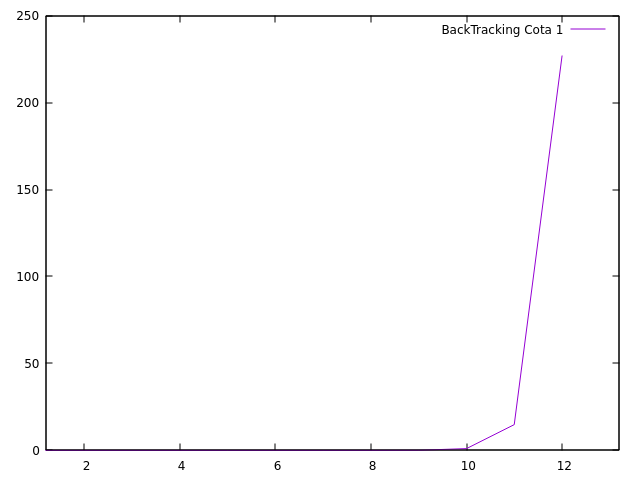
\includegraphics[scale=0.7]{IMAGENES/bt_c1.png}
  	\caption{Primera Cota de BT.}
  	
  \end{center}
\end{figure}

\newpage

\textbf{Segunda Cota}

\begin{table}[h]
    \begin{center}
	\begin{tabular}{|c|c|}
		\hline
		Tamaño & Tiempo \\
		\hline
            1 & 3.386e-06 \\
            2 & 4.426e-06 \\
            3 & 6.581e-06 \\
            4 & 1.5247e-05 \\
            5 & 4.126e-05 \\
            6 & 0.000188035 \\
            7 & 0.00113422 \\
            8 & 0.00717732 \\
            9 & 0.0272816 \\
            10 & 0.275421 \\
            11 & 3.48285 \\
            12 & 45.7452 \\
		\hline
	\end{tabular}
    \end{center}
    \caption{Segunda Cota de BT}
\end{table}
\newpage

\begin{figure}[h]
  \begin{center}
  
  	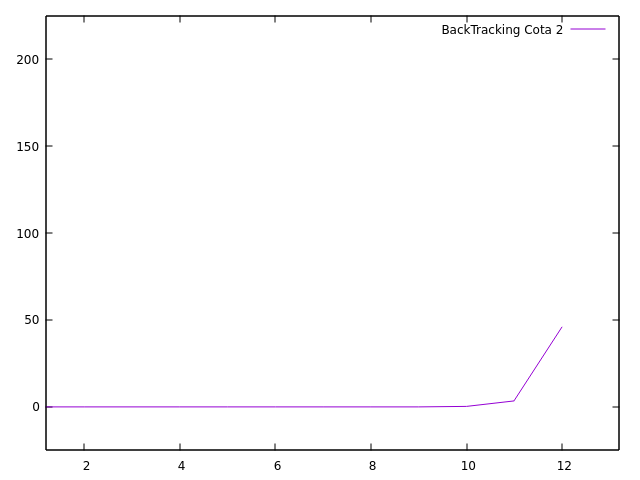
\includegraphics[scale=0.7]{IMAGENES/bt_c2.png}
  	\caption{Segunda Cota de BT.} 
  	
  \end{center}
\end{figure}

\newpage

\textbf{Tercera Cota}
\begin{table}[h]
    \begin{center}
	\begin{tabular}{|c|c|}
		\hline
		Tamaño & Tiempo \\
		\hline
            1 & 4.478e-06 \\
            2 & 6.794e-06 \\
            3 & 1.2591e-05 \\
            4 & 4.2531e-05 \\
            5 & 0.000166765 \\
            6 & 0.00097447 \\
            7 & 0.00500906 \\
            8 & 0.0231318 \\
            9 & 0.181393 \\
            10 & 1.8202 \\
            11 & 22.3786 \\
            12 & 276.022 \\
		\hline
	\end{tabular}
    \end{center}
    \caption{Tercera Cota de BT}
\end{table}

\begin{figure}[h]
  \begin{center}
  
  	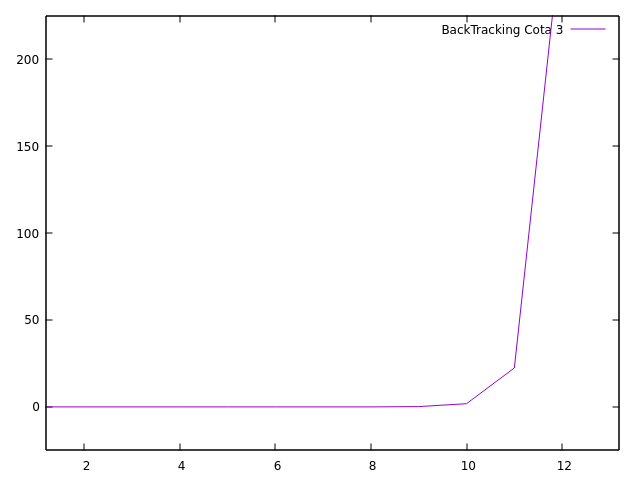
\includegraphics[scale=0.7]{IMAGENES/bt_c3.png}
  	\caption{Tercera Cota de BT.}
  	
  \end{center}
\end{figure}

\newpage

\subsubsection{Análisis Híbrido}
Debido a lo explicado en la sección anterior, no podemos realizar correctamente un análisis híbrido del algoritmo, pues es imposible conocer con exactitud la función a la que se debe ajustar su gráfica.

\newpage

\subsubsection{Análisis Comparativo de Cotas}
\begin{figure}[h]
  \begin{center}
  
  	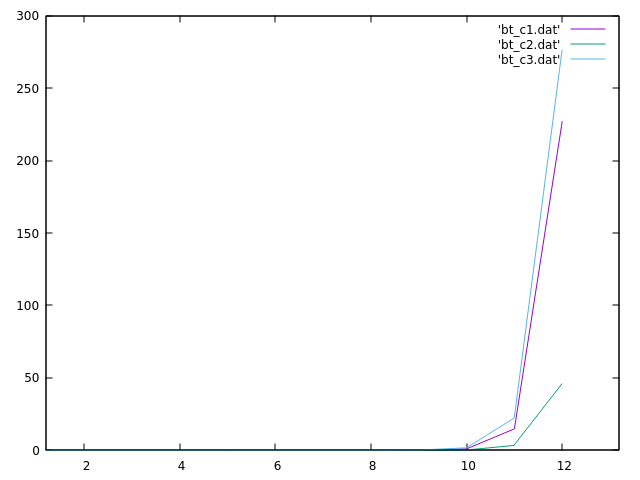
\includegraphics[scale=0.7]{IMAGENES/comparativa_bt.png}
  	\caption{Comparación Cotas.}
  	
  \end{center}
\end{figure}

A partir de esta gráfica podemos concluir que, pasado el umbral de 10 clientes, los tiempos de ejecución se dispara, lo que nos permite afirmar que el algoritmo no es muy eficiente. Aún así, cabe destacar que conseguimos una mejor implementación si usamos la Cota 2.
\newpage


\subsection{Branch and Bound}
Esta técnica combina la exploración de posibles soluciones con la aplicación de límites y restricciones para reducir la cantidad de soluciones a considerar. Para cada nodo del árbol de estados, trata de expandir todos sus hijos antes de explorar cada uno.\\

Para resolver el problema del viajante de comercio con Branch and Bound hemos implementado la clase PVC\_BB:\\

\subsubsection{Implementación}

\lstset{language=C++}

\begin{lstlisting}
/*

 * @brief struct que encapsula el concepto de cliente de un
  vendedor cualquiera.

 * @field x Coordenada x del cliente.

 * @field y Coordenada y del cliente.

 * @field id Identificador del cliente.

 * @field visitado Indicador de si el cliente se ha visitado o no.

 */

struct cliente{

    double x;

    double y;

    int id;

    bool visitado = false; //Restriccion Implicita

    double dist=0;

    double estimador=0;

    vector<cliente> ruta_local;


    /*
     * @brief Sobrecarga del operador de igualdad.
     */

    bool operator== (cliente c1) const{

        return (id==c1.id);

    }

    /*
     * @brief Sobrecarga del operador distinto.
     */

    bool operator!= (cliente c1) const{

        return (id!=c1.id);

    }

};


/*
 *  Functor de comparacion para la ordenacion de la priority_queue.
 */

class comparador {

public:

    bool operator()(const cliente &c1, const cliente &c2) {

        return c1.estimador>c2.estimador;

    }

};


/*
 * @brief Clase que encapsula un entorno de trabajo para el 
 *        Problema del Viajante de Comercio basada en Branch 
 *        and Bound.
 */

class PVC_BB{

private:

    vector<cliente> clientes;

    vector<cliente> ruta_final;

    double cota_global;

    priority_queue<cliente, vector<cliente>,comparador> rutas;

    /*
     * @brief Metodo que calcula la distancia euclidea entre 
     *        dos clientes.
     */

    double distancia(cliente cliente1, cliente cliente2){

        return sqrt(pow(abs(cliente1.x-cliente2.x),2) 
                    + pow(abs(cliente1.y-cliente2.y),2));

    }












   /*
   * @brief Metodo que devuelve la posicion del minimo en una fila 
   *        determinada de una matriz de double.
   * @param matriz_dist Matriz de la que obtener la posicion del 
   *        minimo de la fila.
   * @param pos Fila de la que obtener la posicion del minimo.
   */

    int DevuelveMinimoFila(const vector<vector<double>>& matriz_dist,
                           int pos){

        double min=INFINITY;

        int pos_min = 0;

        for(int i=0;i<matriz_dist[pos].size();++i){

            if(matriz_dist[pos][i]<min && !clientes[i].visitado 
               && i!=pos){

                min = matriz_dist[pos][i];
                pos_min = i;
            }
        }
        return pos_min;
    }















/*
* @brief Metodo que devuelve la posicion del minimo de una 
*        matriz de double.
* @param matriz_dist Matriz de la que obtener la posicion 
*                    del minimo.
*/

int DevuelveMinimoGrafo(const vector<vector<double>>& matriz_dist){

    double min = INFINITY;

    int pos_min = 0;

    for(int i=0; i<matriz_dist.size();++i){

        if(matriz_dist[i][DevuelveMinimoFila(matriz_dist,i)]<min){

            min = 
               matriz_dist[i][DevuelveMinimoFila(matriz_dist,i)];
            pos_min = i;
        }
    }
    return pos_min;
};

public:

   /*
   * @brief Calcula la distancia de una ruta de clientes.
   * @param ruta Vector de clientes del aque calcular la distancia.
   */

    double DistanciaTotal(const vector<cliente>& ruta){

        double sol = 0;

        for(int i=0; i<ruta.size()-1; ++i){
            sol+= distancia(ruta[i],ruta[i+1]);
        }
        return sol;
    }

    /*
     * @brief Contructor con parametros.
     * @param clientes Vector de clientes del que calcular el 
     *                 mejor recorrido.
     */

    PVC_BB (const vector<cliente>& clientes){

        this->clientes=clientes;

        ruta_final=clientes;

        cota_global= DistanciaTotal(clientes) + 
        distancia(clientes[0],clientes[clientes.size()-1]);

    }

     /*
     * @brief Metodo que crea una matriz de distacias a partir 
     *        de un vector de clientes.
     * @param clientes Vector de clientes del que calcular 
     *        calcular las distancias de todos los clientes 
     *        con todos.
     */
    vector<vector<double>> CrearMatriz(const vector<cliente>& clientes){

        vector<vector<double>> matriz_dist= 
        vector<vector<double>>(clientes.size(),
                               vector<double>(clientes.size()));

        for(int i=0;i<clientes.size();++i){
            for(int j=0;j<clientes.size();++j){
                matriz_dist[i][j]= distancia(clientes[i],clientes[j]);
            }
        }

        return matriz_dist;
    }


    /*
     * @brief Devuelve el vector ruta solucion.
     */

    vector<cliente> getRutaFinal(){

        return this->ruta_final;

    }


    /*
     * @brief Devuelve la cota global de la ruta.
     */

    double getCotaGlobal(){return this->cota_global;}

    /*
    * @brief Algoritmo basado en Branch and Bound para el Problema 
    *        del Viajante de Comercio.
    * @param matriz_dist Matriz de distancias de los clientes.
    * @param Cota Funcion que determina la optimalidad de las 
    *        soluciones que se van calculando.
    * @param Matriz de double que se correspondera con la matriz 
    *        de distancias.
    * @param Cliente (nodo) del cual se comprobara la optimalidad 
    *        de su ruta parcial.
    */

    void BB(const vector<vector<double>>& matriz_dist,
            double (PVC_BB::*Cota)(const vector<vector<double>>&,
                                   cliente)) {

        cliente raiz=clientes[0];
        raiz.ruta_local.push_back(clientes[0]);
        raiz.visitado=true;
        clientes[0].visitado=true;
        rutas.push(raiz);



        while (!rutas.empty()){

            cliente cliente_actual=rutas.top();

            rutas.pop();

            for(int i=0;i<clientes.size();++i){

                clientes[i].visitado=false;

            }

            for(int i=0;i<cliente_actual.ruta_local.size();++i){

                clientes[cliente_actual.ruta_local[i].id].visitado=true;

            }

              if (cliente_actual.ruta_local.size()==clientes.size()){

                cliente_actual.dist+= matriz_dist[cliente_actual.id][0]; //Volver al inicio

               if (cliente_actual.dist < cota_global) {

                   cota_global = cliente_actual.dist;

                   ruta_final = cliente_actual.ruta_local;

               }

            }

            else{

                for (int i=1; i<clientes.size();i++) {

                    if (!clientes[i].visitado && clientes[i] 
                        != cliente_actual) {

                        cliente hijo;

                    hijo.ruta_local = cliente_actual.ruta_local;

                    hijo.ruta_local.push_back(clientes[i]);

                    hijo.dist = cliente_actual.dist +
                                matriz_dist[i][cliente_actual.id];

                    hijo.x = clientes[i].x;

                    hijo.y = clientes[i].y;

                    hijo.id = clientes[i].id;

                    hijo.estimador=(this->*Cota)(matriz_dist,hijo);

                    if (cota_global>hijo.estimador) {

                        rutas.push(hijo);

                    }

                }

            }

        }

    }

  }

};



\end{lstlisting}

\vspace{1cm}

\newpage

\subsubsection{Funciones de cota}

\textbf{Primera Cota}

 Para esta primera cota elegimos como cota local el resultado de multiplicar el peso del menor arco por el número de ciudades que quedan por visitar, y a eso sumarle la distancia recorrida hasta el momento. Lo hemos implementado de la siguiente manera:

\lstset{language=C++}
\begin{lstlisting}

    /*
     * @brief Primer estimador para determinar la validez de las 
       posibles soluciones a lo largo de su construccion.
     * Selecciona el arco de menor peso y multiplica dicho peso por 
       el numero de ciudades que quedan por visitar.
     * @param matriz_dist Matriz de distancias.
     * @param nodo Nodo del que tomamos los datos del momento.
     */

double FuncionCota1(const vector<vector<double>>& matriz_dist,
                     cliente nodo){

    double menor_peso=
        matriz_dist[DevuelveMinimoGrafo(matriz_dist)]
       [DevuelveMinimoFila(matriz_dist,
                           DevuelveMinimoGrafo(matriz_dist))];

    int quedan_por_visitar=clientes.size()-nodo.ruta_local.size();

    return (menor_peso*quedan_por_visitar)+nodo.dist;

}
\end{lstlisting}

\newpage
\textbf{Segunda Cota}

 A continuación, hemos creado la siguiente función para asignar a la cota local el resultado de sumarle a la distancia recorrida hasta el momento el mínimo valor de "salir" de cada nodo aún no visitado. La implementación es la siguiente:
 
\lstset{language=C++}
 \begin{lstlisting}
 
    /*
     * @brief Segundo estimador para determinar la validez de las 
       posibles soluciones a lo largo de su construccion.
     * Selecciona el arco de menor peso al salir de todos los
       nodos restantes por visitar, y suma esto a la distancia
     * acumulada del camino ya recorrido.
     * @param matriz_dist Matriz de distancias.
     * @param nodo Nodo del que tomamos los datos del momento.
     */

double FuncionCota2(const vector<vector<double>>& matriz_dist,
                   cliente nodo){

    double dist_acumulada=nodo.dist;

    for (int i=0; i<matriz_dist.size();++i){

        if (!clientes[i].visitado && i!=nodo.id) {

             dist_acumulada+=matriz_dist[i]
             [DevuelveMinimoFila(matriz_dist,i)];

        }

    }

    return dist_acumulada;

}


\end{lstlisting}

\newpage
\textbf{Tercera Cota}

Para la tercera y última función se ha seguido el siguiente criterio: para cada arista se considera la mitad de su peso como el costo de salir y entrar, y, para las ciudades que aún no han sido visitadas, se considera la mitad de la suma de sus dos menores arcos. Lo hemos implementado como sigue

\lstset{language=C++}
\begin{lstlisting}
  /*
    * @brief Tercer estimador para determinar la validez de las
      posibles soluciones a lo largo de su construccion.
    * Selecciona el arco de menor peso al salir y entrar en cada 
      nodo, dividiendo por 2.
    * @param matriz_dist Matriz de distancias.
    * @param nodo Nodo del que tomamos los datos del momento.
    */

double FuncionCota3(const vector<vector<double>>& matriz_dist,
    cliente nodo){

    vector<vector<double>> m=matriz_dist;

    double aux=0;
    
    double d=0;
    
    double min1;

    if(nodo.ruta_local.size()==1) {

        min1=matriz_dist[nodo.ruta_local[0].id]
        [DevuelveMinimoFila(matriz_dist,nodo.ruta_local[0].id)];

         m[nodo.ruta_local[0].id]
         [DevuelveMinimoFila(matriz_dist,nodo.ruta_local[0].id)]=
         INFINITY;

         d=(min1 + m[nodo.ruta_local[0].id]
         [DevuelveMinimoFila(m,nodo.ruta_local[0].id)])/2;

    }


    else{

        aux=matriz_dist[nodo.ruta_local[0].id]
        [DevuelveMinimoFila(matriz_dist,nodo.ruta_local[0].id)];

        for(int i=0;i<nodo.ruta_local.size()-1;++i){

            d+=((aux+distancia(nodo.ruta_local[i],
            nodo.ruta_local[i+1]))/2);

            aux=distancia(nodo.ruta_local[i],
                          nodo.ruta_local[i+1]);
         }

        d+=(aux+matriz_dist[nodo.ruta_local.back().id]
        [DevuelveMinimoFila(matriz_dist,nodo.ruta_local.back().id)])
        /2;

        for (int i=0; i<matriz_dist.size();++i) {

            if(!clientes[i].visitado && i!=nodo.id) {

                 min1=matriz_dist[i]
                 [DevuelveMinimoFila(matriz_dist,i)];

                 m[i][DevuelveMinimoFila(matriz_dist,i)]=INFINITY;

                d+=(min1 + m[i][DevuelveMinimoFila(m,i)])/2;

            }

        }

    }

    return d;

}


\end{lstlisting}

\newpage

\subsubsection{Análisis Teórico}
Podemos comprobar que Branch and Bound ofrece una solución exacta a un problema tipo NP-completo. Sin embargo, no es posible determinar con exactitud su eficiencia teórica, pues depende de la cota utilizada y la profundidad del árbol de estados.\\
\newpage

\subsubsection{Análisis Empiríco}
\vspace{0.5cm}

\textbf{Primera Cota}

\begin{table}[h]
    \begin{center}
	\begin{tabular}{|c|c|}
		\hline
		Tamaño & Tiempo \\
		\hline
            1 & 3.105e-06 \\
            2 & 6.942e-06 \\
            3 & 1.2586e-05 \\
            4 & 2.9624e-05 \\
            5 & 8.2204e-05 \\
            6 & 0.000314677 \\
            7 & 0.00137956 \\
            8 & 0.00491169 \\
            9 & 0.0125177 \\
            10 & 0.100669 \\
            11 & 0.250452 \\
            12 & 1.02855 \\
            13 & 4.22054 \\
            14 & 10.5575 \\
            15 & 79.4179 \\	
		\hline
	\end{tabular}
    \end{center}
    \caption{Primera Cota de BB}
\end{table}
\newpage

\begin{figure}[h]
  \begin{center}
  
  	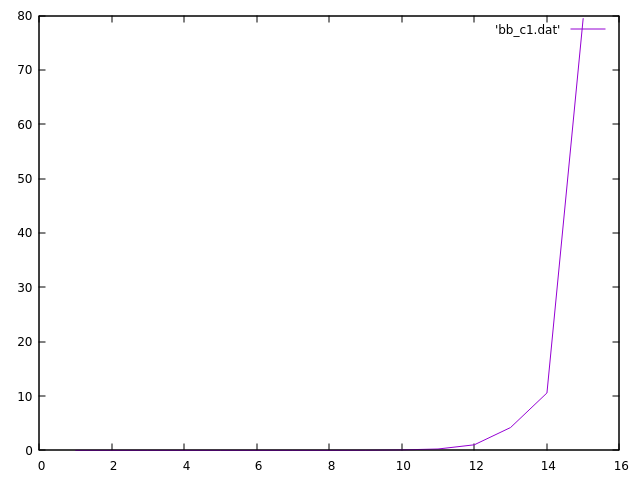
\includegraphics[scale=0.7]{IMAGENES/bb_c1.png}
  	\caption{Primera Cota de BB.}
  	
  \end{center}
\end{figure}
\newpage

\textbf{Segunda Cota}

\begin{table}[h]
    \begin{center}
	\begin{tabular}{|c|c|}
		\hline
		Tamaño & Tiempo \\
		\hline
            1 & 2.151e-06 \\
            2 & 5.999e-06 \\
            3 & 2.3176e-05 \\
            4 & 2.628e-05 \\
            5 & 5.7239e-05 \\
            6 & 0.00015582 \\
            7 & 0.000571988 \\
            8 & 0.00408475 \\
            9 & 0.00677485 \\
            10 & 0.0139719 \\
            11 & 0.0147906 \\
            12 & 0.0666161 \\
            13 & 0.0994902 \\
            14 & 0.256098 \\
            15 & 0.221284 \\
		\hline
	\end{tabular}
    \end{center}
    \caption{Segunda Cota de BB}
\end{table}
\newpage

\begin{figure}[h]
  \begin{center}
  
  	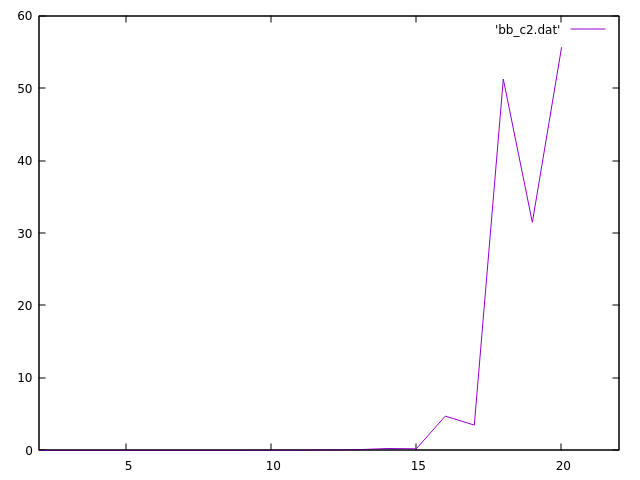
\includegraphics[scale=0.7]{IMAGENES/bb_c2.png}
  	\caption{Segunda Cota de BB}
  	
  \end{center}
\end{figure}
\newpage

\textbf{Tercera Cota}

\begin{table}[h]
    \begin{center}
	\begin{tabular}{|c|c|}
		\hline
		Tamaño & Tiempo \\
		\hline
            1 & 2.414e-06 \\
            2 & 8.09e-06 \\
            3 & 1.1687e-05 \\
            4 & 3.4637e-05 \\
            5 & 4.4661e-05 \\
            6 & 0.000272908 \\
            7 & 0.000601703 \\
            8 & 0.000305369 \\
            9 & 0.00093021 \\
            10 & 0.00383178 \\
            11 & 0.0105167 \\
            12 & 0.00905677 \\
            13 & 0.145045 \\
            14 & 0.0421317 \\
            15 & 0.604139 \\
		\hline
	\end{tabular}
    \end{center}
    \caption{Tercera Cota de BB}
\end{table}
\newpage
\begin{figure}[h]
  \begin{center}
  
  	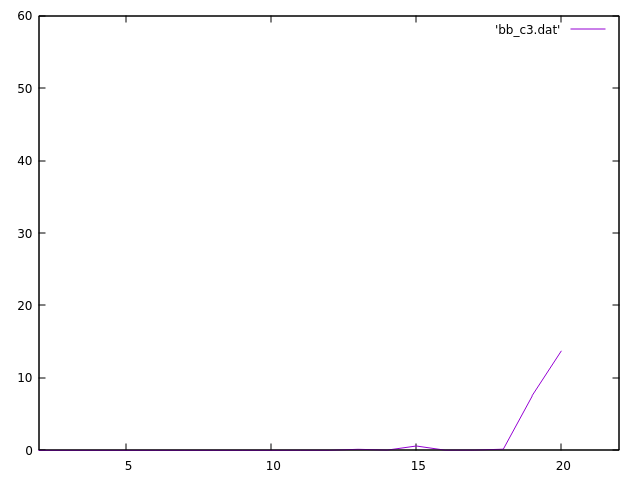
\includegraphics[scale=0.7]{IMAGENES/bb_c3.png}
  	\caption{Tercera Cota de BB.}
  	
  \end{center}
\end{figure}
\newpage

\subsubsection{Análisis Híbrido}
Debido a lo explicado en la sección anterior, no podemos realizar correctamente un análisis híbrido del algoritmo, pues es imposible conocer con exactitud la función a la que se debe ajustar su gráfica.

\subsubsection{Análisis Comparativo de Cotas}

\begin{figure}[h]
  \begin{center}
  
  	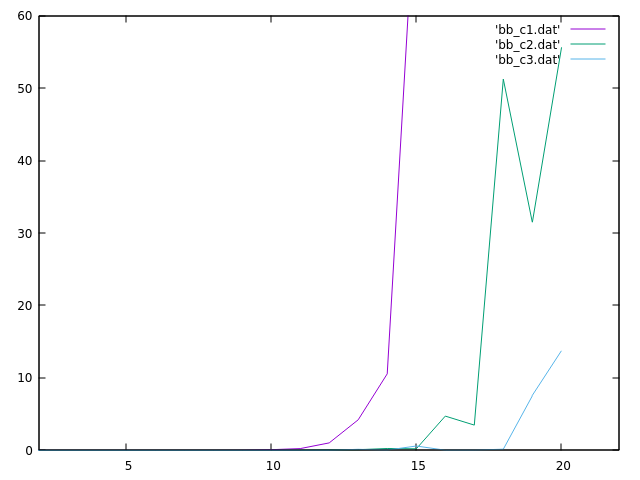
\includegraphics[scale=0.7]{IMAGENES/comparativa_bb.png}
  	\caption{Comparación Cotas de BB.}
  	
  \end{center}
\end{figure}

A partir de esta gráfica podemos ver que como los tiempos de ejecución se disparan súbitamente en cada cota a pesar de ser muy eficientes en casos muy pequeños. Aún así, observamos claramente la considerable diferencia en cuanto a eficiencia de la Cota 3, que incluso llega a ejecutarse para 20 clientes en menos de la mitad del tiempo que las cotas restantes.
\newpage

\subsection{Análisis Comparativo entre BB y BT}


\begin{figure}[h]
  \begin{center}
  
  	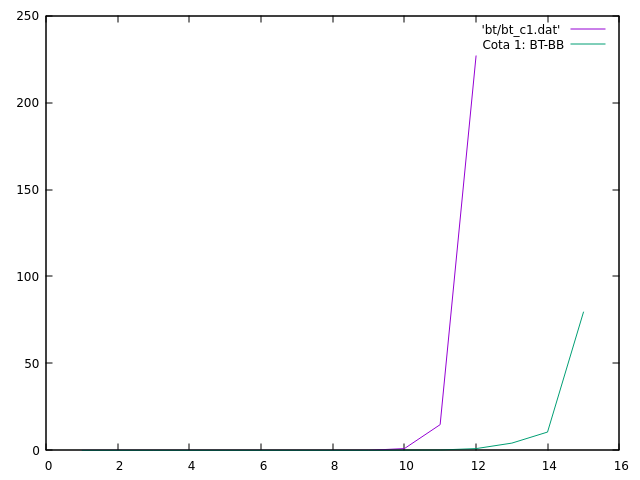
\includegraphics[scale=0.7]{IMAGENES/bt_bb_c1.png}
  	\caption{Comparación Cota 1}
  	
  \end{center}
\end{figure}
\newpage
\begin{figure}[h]
  \begin{center}
  
  	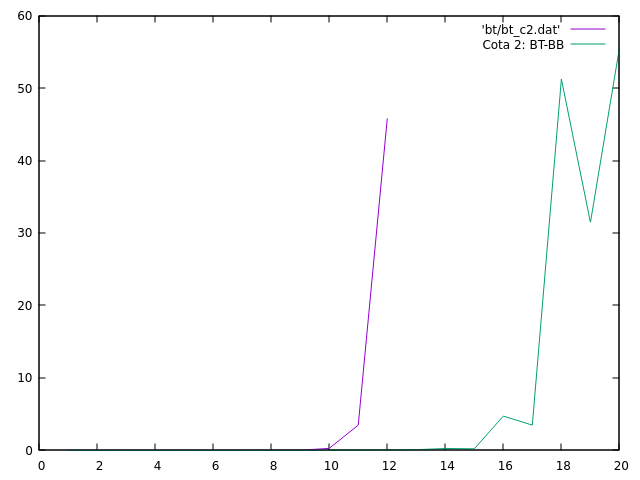
\includegraphics[scale=0.7]{IMAGENES/bt_bb_c2.png}
  	\caption{Comparación Cota 2}
  	
  \end{center}
\end{figure}
\newpage
\begin{figure}[h]
  \begin{center}
  
  	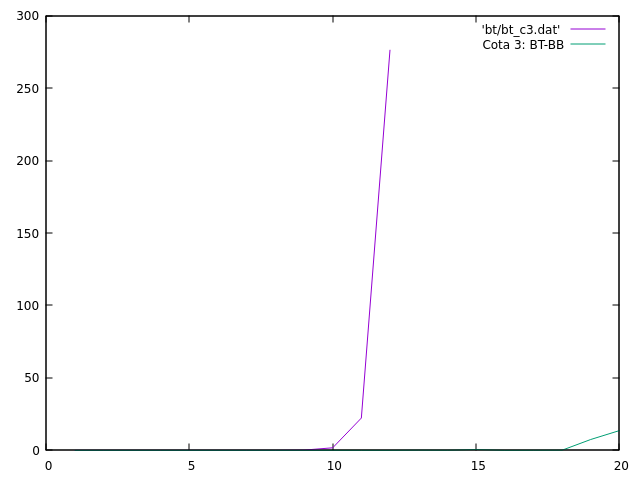
\includegraphics[scale=0.7]{IMAGENES/bt_bb_c3.png}
  	\caption{Comparación Cota 3}
  	
  \end{center}
\end{figure}

Así, vemos que para las tres cotas observamos que el branch and bound nos proporciona unas soluciones más eficiente aún usando las mismas funciones de cota, lo que se debe a que, mientras que la técnica BackTracking realiza una búsqueda exhaustiva en la que crea todas las soluciones posibles, la poda del Branch and Bound permite ahorrar permutaciones.
\newpage

\section{Conclusiones} 

\begin{itemize}
	\item La dificultad que supone la implementación de esta clase de algoritmos y su coste computacional.
	\item La versatilidad que ofrecen la técnicas \textit{Backtracking} y \textit{Branch and Bound} para la resolución de problemas.
	\item Las diferencias en eficiencia y complejidad que suponen las distintas técnicas de exploración de grafos.
 \item La importancia de realizar funciones de cota óptimas y su repercusión en la eficiencia del código final.

\end{itemize}

\end{document}